\documentclass{article}
\usepackage{tikz}
\usepackage{float}
\usepackage{enumerate}
\usepackage{amsmath}
\usepackage{amsthm}
\usepackage{bm}
\usepackage{indentfirst}
\usepackage{siunitx}
\usepackage[utf8]{inputenc}
\usepackage{graphicx}
\graphicspath{ {Images/} }
\usepackage{float}
\usepackage{mhchem}
\usepackage{chemfig}
\allowdisplaybreaks

\title{6.041 Problem Set 11}
\author{Robert Durfee - R02}
\date{November 21, 2018}

\begin{document}

\maketitle

\section*{Problem 1}

\subsection*{Part A}

Let $R_i$ represent the event that both Alice and Bob lose on round $i$. The
probability of this event is given by the product of the probability of each
losing from the PMF of $G$.
$$ P(R_i) = p_G(-2)^2 = \left(\frac{1}{3}\right)^2 = \frac{1}{9} $$
Now, the number of rounds up to \textit{and including} the first round in
which both Alice and Bob lose is given by the geometric distribution with
parameter $p = 1/9$.
$$ p_X(k) = \left(1 - \frac{1}{9}\right)^{k - 1} \left(\frac{1}{9}\right) $$

\subsection*{Part B}

Once again, segregate the plays into rounds. Let $R_i$ now represent the
event that Bob loses in round $i$. This is given from the PMF of $G$.
$$ P(R_i) = p_G(-2) = \frac{1}{3} $$
Now, the event $Y$ is defined as the third loss. This is the same as the
$k$th arrival of a loss where $k = 3$. Therefore, the PMF follows that seen
in lecture,
$$ p_{Y_k}(t) = \binom{t - 1}{k - 1} p^k (1 - p)^{t - k}\quad t \in \{k, k +
1, \ldots\} $$
$$ p_{Y_3}(t) = \binom{t - 1}{2} \left(\frac{1}{3}\right)^3 \left(1 -
\frac{1}{3}\right)^{t - 3} \quad t \in \{3, 4, \ldots\} $$
However, the $t$ is in terms of rounds rather than times. Therefore, the PMF
in terms of times is given by $t' = 2t$
$$ p_{Y_3}(t') = \binom{t'/2 - 1}{2} \left(\frac{1}{3}\right)^3 \left(1 -
\frac{1}{3}\right)^{t'/2 - 3} \quad t' \in \{6, 8, \ldots \} $$

\subsection*{Part C}

There are four cases to consider
\begin{itemize}
  \item $A_1$: Only Alice wins the first round.
  \item $A_2$: Only Bob wins the first round.
  \item $A_3$: Both Alice and Bob win the first round.
  \item $A_4$: Neither Alice nor Bob win the first round.
\end{itemize}
From this, the expectation of number of rounds until each has won once is
given by the Law of Total Expectation
$$ E[N] = \sum_{i = 1}^4 P(A_i) E[N \mid A_i] $$
From the definition of a geometric distribution, the individual conditional
expectations follow, where $p$ is the probability of a loss for either Alice
or Bob at a given play.
$$ E[N \mid A_1] = E[N \mid A_2] = 1 + \frac{1}{1 - p} $$
$$ E[N \mid A_3] = 1 $$
$$ E[N \mid A_4] = 1 + E[N] $$
Therefore, combined with the probabilities from the PMF for $G$, the total
expectation is
$$ E[N] = 2 p (1 - p) \left(1 + \frac{1}{1 - p}\right) + p^2 + (1 - p)^2 (1 +
E[N]) $$
Solving for $E[N]$ after substituting $p = 2/3$ yields,
$$ E[N] = \frac{15}{8} $$

\section*{Problem 2}

\subsection*{Part A}

Given that the widget was sold, it is known that the price it sold for is
greater than $2$. Therefore, the PDF is given conditioned on $z \geq 2$.
Using the definition of conditional probability,
$$ P(Z = z \mid Z \geq 2) = \frac{P(Z = z \cap Z \geq 2)}{P(Z
\geq 2)} \quad z \in [0, \infty) $$
This can be simplified to the following by realizing that the numerator is
$0$ when $z \in [0, 2]$.
$$ P(Z = z \mid Z \geq 2) = \frac{P(Z = z)}{P(Z \geq 2)} \quad
z \in [2, \infty) $$
Written in terms of the provided PDFs,
$$ P(Z = z \mid Z \geq 2) = \frac{f_{Z}(z)}{1 - F_{Z}(2)} = 2
e^{4 - 2z} \quad z \in [2, \infty) $$

\begin{center}
    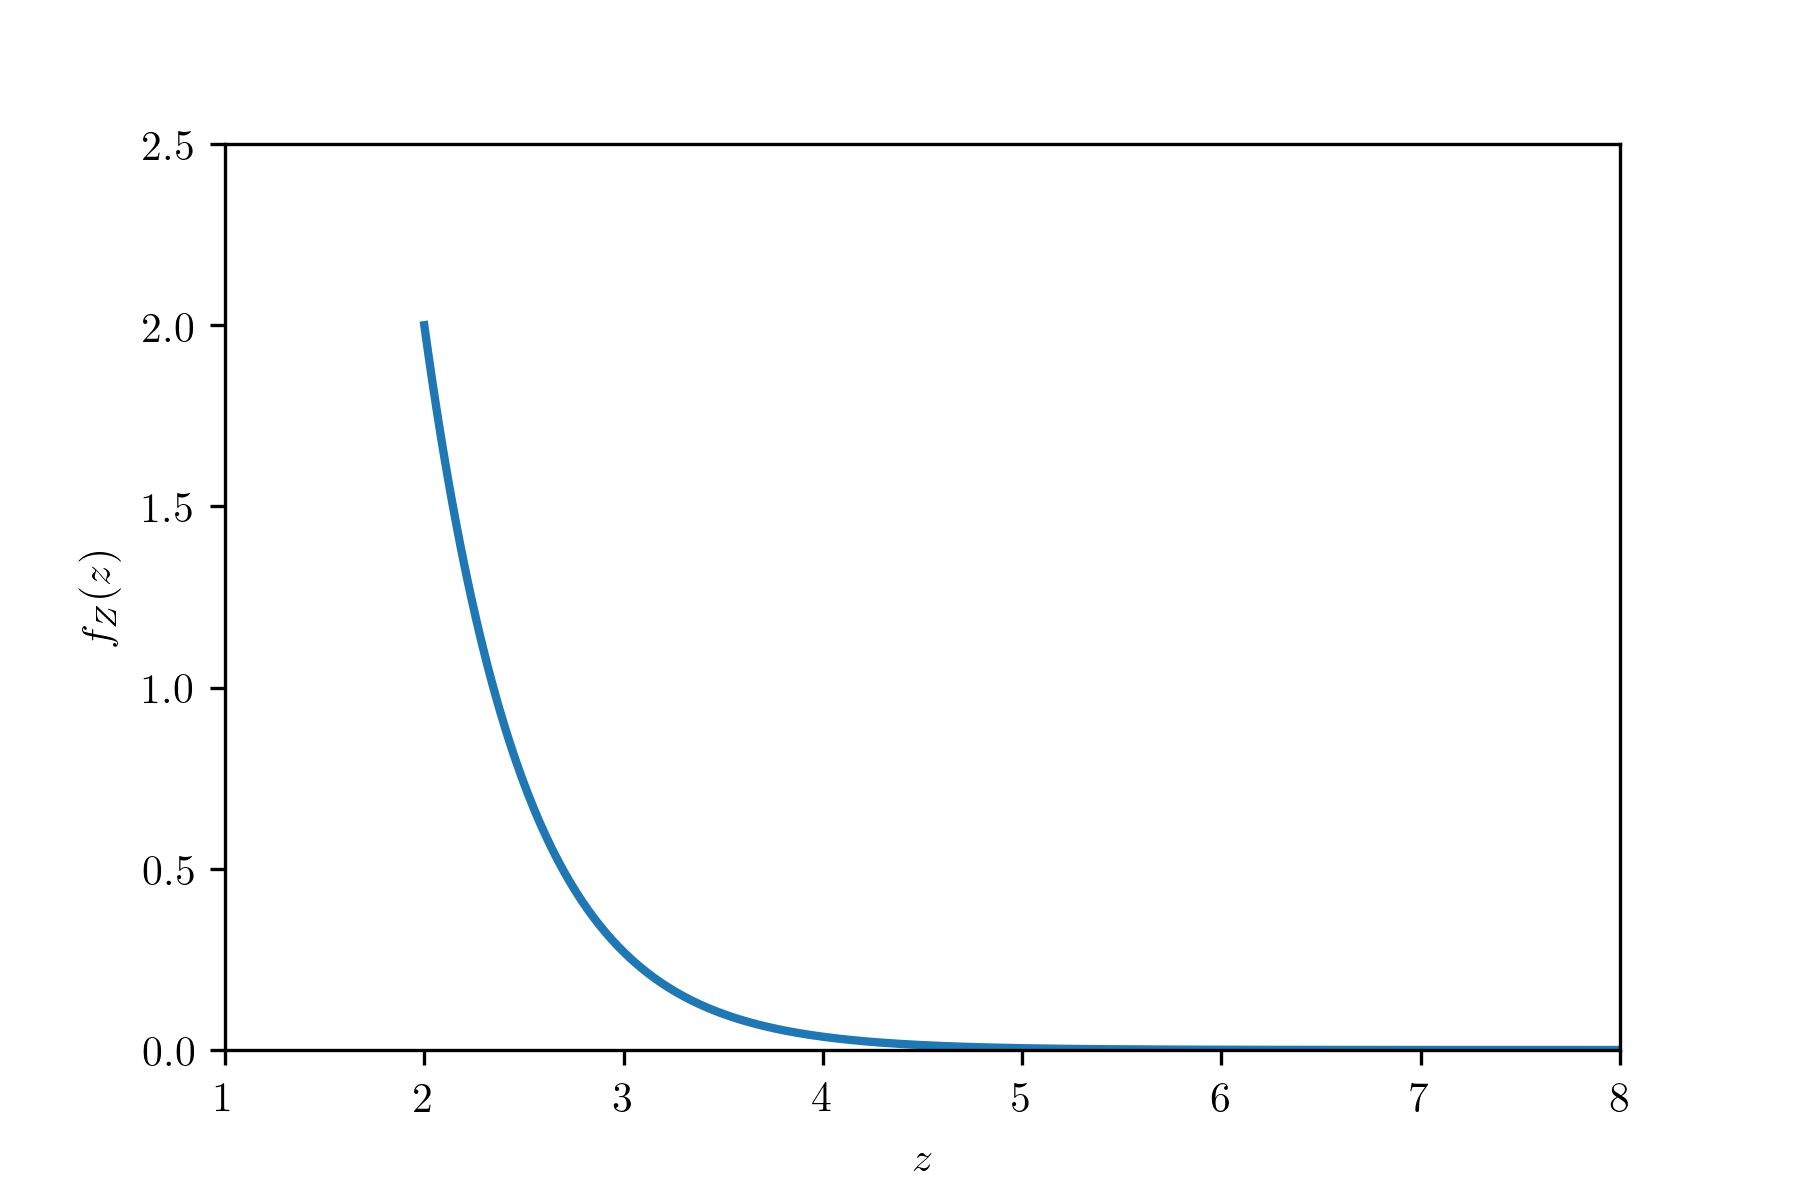
\includegraphics[scale=0.85]{Images/P2a.PNG}
\end{center}

\subsection*{Part B}

Yes, $X_1, X_2, X_3, \ldots$ is a Bernoulli process. There are only two
possible outcomes for each $X_i$: either the widget sold or it wasn't.
Furthermore, each outcome is independent from the rest as the selling is
conditioned upon a fixed constant. Lastly, the probability of succes for each
$X_i$ is shared between all $X_i$ and remains constant.

\subsection*{Part C}

The probability that Rajeev makes his third sale on Day 10 is equivalent to
saying the $k$th arrival of his sale happens at time $t$ where $k = 3$ and $t
= 10$. Therefore, the $k$th arrival PMF can be used from lecture,
$$ p_{Y_k}(t) = \binom{t - 1}{k - 1} p^k (1 - p)^{t - k} \quad t \in \{k, k +
1, \ldots \}$$
Substituting $k$ and $t$ and the probability that $z \geq 2$ calculated in
Part A,
$$ p_{Y_3}(10) = \binom{9}{2} \left(e^{-4}\right)^3 \left(1 -
e^{-4}\right)^{7} \approx 1.94 \cdot 10^{-4} $$

\subsection*{Part D}

Let $S = Z_2 - Z_1$. The PDF for $S$ can be determined through convolution,
$$ f_S(s) = \int_{-\infty}^\infty f_{Z_2}(t) f_{Z_1}(t - s) dt $$
The limits are given by $t \in [0, \infty)$, $t - s \in [2, \infty)$, and $s
\in (-\infty, \infty)$. Therefore, the integral becomes piecewise,
$$ f_S(s) = \begin{cases}
  \int_0^\infty f_{Z_2}(t) f_{Z_1}(t - s) dt & s \in (-\infty, -2] \\
  \int_{2 + s}^\infty f_{Z_2}(t) f_{Z_1}(t - s) dt & s \in [-2, \infty)
\end{cases} $$
Evalutating the integrals yields,
$$ f_S(s) = \begin{cases}
  e^{2(s + 2)} & s \in (-\infty, -2] \\
  e^{-2(s + 2)} & s \in [-2, \infty)
\end{cases} $$

\subsection*{Part E}

Let $R_1$ be the first record high and $R_2$ be the second. The conditional
probability of $R_2$ given $R_1$ can be written as follows, given that $R_2$
must be greater than the previous $R_1$,
$$ P(R_2 = r_2 \mid R_2 > r_1) = \frac{P(R_2 = r_2 \cap R_2 > r_1)}{P(R_2 >
r_1)} \quad r_1 \in [0, \infty), r_2 \in [0, \infty) $$
Simplifying the same as in Part A,
$$ P(R_2 = r_2 \mid R_2 > r_1) = \frac{P(R_2 = r_2)}{P(R_2 > r_1)} \quad r_1
\in [0, \infty), r_2 \in [r_1, \infty) $$
Written using PDF notation,
$$ f_{R_2|R_1}(r_2 \mid r_1) = \frac{f_{R_2}(r_2)}{1 - F_{R_2}(r_1)} \quad
r_1 \in [0, \infty), r_2 \in [r_1, \infty) $$
Substituting the PDFs yields,
$$ f_{R_2|R_1}(r_2 \mid r_1) = 2 e^{2(r_1 - r_2)} \quad r_1 \in [0, \infty),
r_2 \in [r_1, \infty) $$
From the definition of expectation, the conditional expectation of $R_2$
given $R_1$ is
\begin{align*}
  E[R_2 \mid R_1 = r_1] &= \int_{-\infty}^{\infty} r_2 f_{R_2|R_1}(r_2 \mid
  r_1) dr_{2} \\
  &= \int_{r_1}^{\infty} r_2 2 e^{2(r_1 - r_2)} dr_2 \\
  &= r_1 + \frac{1}{2} 
\end{align*}
Using total expectation, the expected value of $R_2$ can be determined,
\begin{align*}
  E[R_2] &= \int_{-\infty}^{\infty} f_{R_1}(r_1) E[R_2 \mid R_1 = r_1] dr_1 \\
  &= \int_0^{\infty} \left(2e^{-2r_1}\right) \left(r_1 + \frac{1}{2}\right)
  dr_1 \\
  &= 1
\end{align*}

\subsection*{Part F}

Let $R_i$ be the $i$th record high. The conditional probability of $R_i$
given $R_{i - 1}, R_{i - 2}, \ldots, R_{1}$ can be written as follows
$$ P(R_i = r_i \mid R_{i - 1} = r_{i - 1}, R_{i - 2} = r_{i - 2}, \ldots, R_1
= r_1) $$
However, not all the previous values are important as they are all strictly
increasing. Therefore, this simplifies to
$$ P(R_i = r_i \mid R_{i - 1} = r_{i - 1}) $$
Which, as shown before, takes the form,
$$ f_{R_i|R_{i - 1}}(r_i \mid r_{i-1}) = 2 e^{2(r_{n - 1} - r_n)} $$
Furthermore, it is clear that the conditional expected value is also the same,
$$ E[R_n \mid R_1^{n - 1}] = E[R_n \mid R_{n - 1}] = r_{n - 1} + \frac{1}{2} $$
Once again, using the Law of Total Expectation,
$$ E[R_n] = \int_{-\infty}^\infty f_{R_1^{n-1}}\left(r_1^{n-1}\right)
E\left[R_n \mid R_1^{n - 1}\right] dr_1^{n - 1} $$
Using the multiplication rule, the joint PDF $f_{R_1^{n - 1}}\left(r_1^{n -
1}\right)$ can be determined as follows,
$$ f_{R_1^{n - 1}}\left(r_1^{n - 1}\right) = \left(2 e^{-2r_1}\right) \left(2
e^{2(r_1 - r_2)}\right) \ldots \left(2 e^{2(r_{n - 2} - r_{n - 1})}\right) =
2^{n - 1} e^{-2r_{n - 1}} $$
Substituting into the Law of Total Expectation as described earlier,
$$ E[R_n] = \int_0^\infty 2^{n - 1} e^{-2r_{n - 1}} \left(r_{n - 1} +
\frac{1}{2}\right) dr_{n - 1} = 2^{n - 2}$$

\subsection*{Part G}

The process $Y_1, Y_2, Y_3, \ldots$ cannot be a Bernoulli process because the
first record high is deterministic: it must occur at $Z_1$. Therefore, $P(Y_1
= 1) = 1$. This does not remain true through the rest of the process. Thus
there is no common $p$ for the process.

\subsection*{Part H}

First, we must determine the probability that $Y_i = 1$ for $i > 1$. This
will occur when $Z_i > R_1$. Looking at the conditional probability,
$$ P(Z_i > R_1 \mid R_1 = r_1) = P(Z_i > r_1) = 1 - F_{Z_i}(r_1) = e^{-2 r_1} $$
Using the Law of Total Probability,
\begin{align*}
  P(Z_i > R_1) &= \int_{-\infty}^{\infty} f_{R_1}(r_1) P(Z_i > R_1 \mid R_1 =
  r_1) dr_1 \\
  &= \int_0^{\infty} \left(2 e^{-2r_1}\right) \left(e^{-2 r_1}\right) dr_1 \\
  &= \frac{1}{2}
\end{align*}
Using this parameter in the Pascal distribution for the \textit{first}
arrival time (as the real first arrival is deterministic), the second arrival
time is given by
$$ p_{Y_2}(t) = \left(\frac{1}{2}\right) \left(1 - \frac{1}{2}\right)^{t - 1} $$
However, the first time slot is occupied by the deterministic $Y_1$,
therefore $t' = t + 1$. Substituting into the above expression,
$$ p_{Y_2}(t') = \left(\frac{1}{2}\right) \left(1 - \frac{1}{2}\right)^{t' -
2} $$

\end{document}